\section{Methodik}

\subsection{Beschreibung der Datenquelle und -beschaffung}

\subsection{Beschreibung der Algorithmen}
Der Studiengangsfinder soll Studieninteressierten einen schnellen Überblick über
alle in Frage kommenden Studiengänge ermöglichen.  Dabei soll dem Nutzer eine
interaktive Grafik präsentiert werden, mit der er anhand von Studieninhalten
(z.B. \glqq Gesundheit und Soziales\grqq{}) sofort alle relevanten Studiengänge
findet. Dazu ist es notwendig, die Studiengänge nach ihren Inhalten zu
gruppieren (Clustering) und schließlich visuell ästhetisch aufzubereiten.

Bei der Festlegung des Clustering-Algorithmus für den Studiengangfinder wurden
verschiedene Optionen in Betracht gezogen, darunter K-Means Clustering,
Force-Directed Layouts und Multidimensionale Skalierung (MDS). Nach einer
gründlichen Abwägung der Vor- und Nachteile fiel die Wahl auf MDS. Die Gründe
für diese Entscheidung und eine Erläuterung der jeweiligen Algorithmen werden in
den folgenden Kapiteln gegeben.

\subsubsection{Force-Directed-Graphs}
Force-Directed Graph Drawing ist eine Methode zur Visualisierung von Graphen,
bei der die Positionen der Knoten und Kanten aufgrund von Kräften bestimmt
werden. Das Vorgehen hierbei ist vereinfacht inspiriert von Modellen der
Teilchenphysik und wird häufig mit dem Verhalten von Federn verglichen. Ziel des
Algorithmus ist es durch Kanten verbundene Knoten nah beinander zu platzieren
und somit eine ästhetisch ansprechende Visualisierung eines Graphen zu
berechnen. In \autoref{fig:force-directed-layouts} erkennt man ausgehend von
einer zufälligen Positionierung (Zustand 0), eine schrittweise Optimierung der
Darstellung. Wie stark oder schwach sich die Knoten jeweils
\glqq anziehen\grqq{} bzw. \glqq abstoßen\grqq{} wird durch die Gleichmäßigkeit
der Verteilung auf der sogenannten Zeichenfläche bestimmt.
\parencite{force-directed-layouts}

\begin{figure}[H]
    \centering
    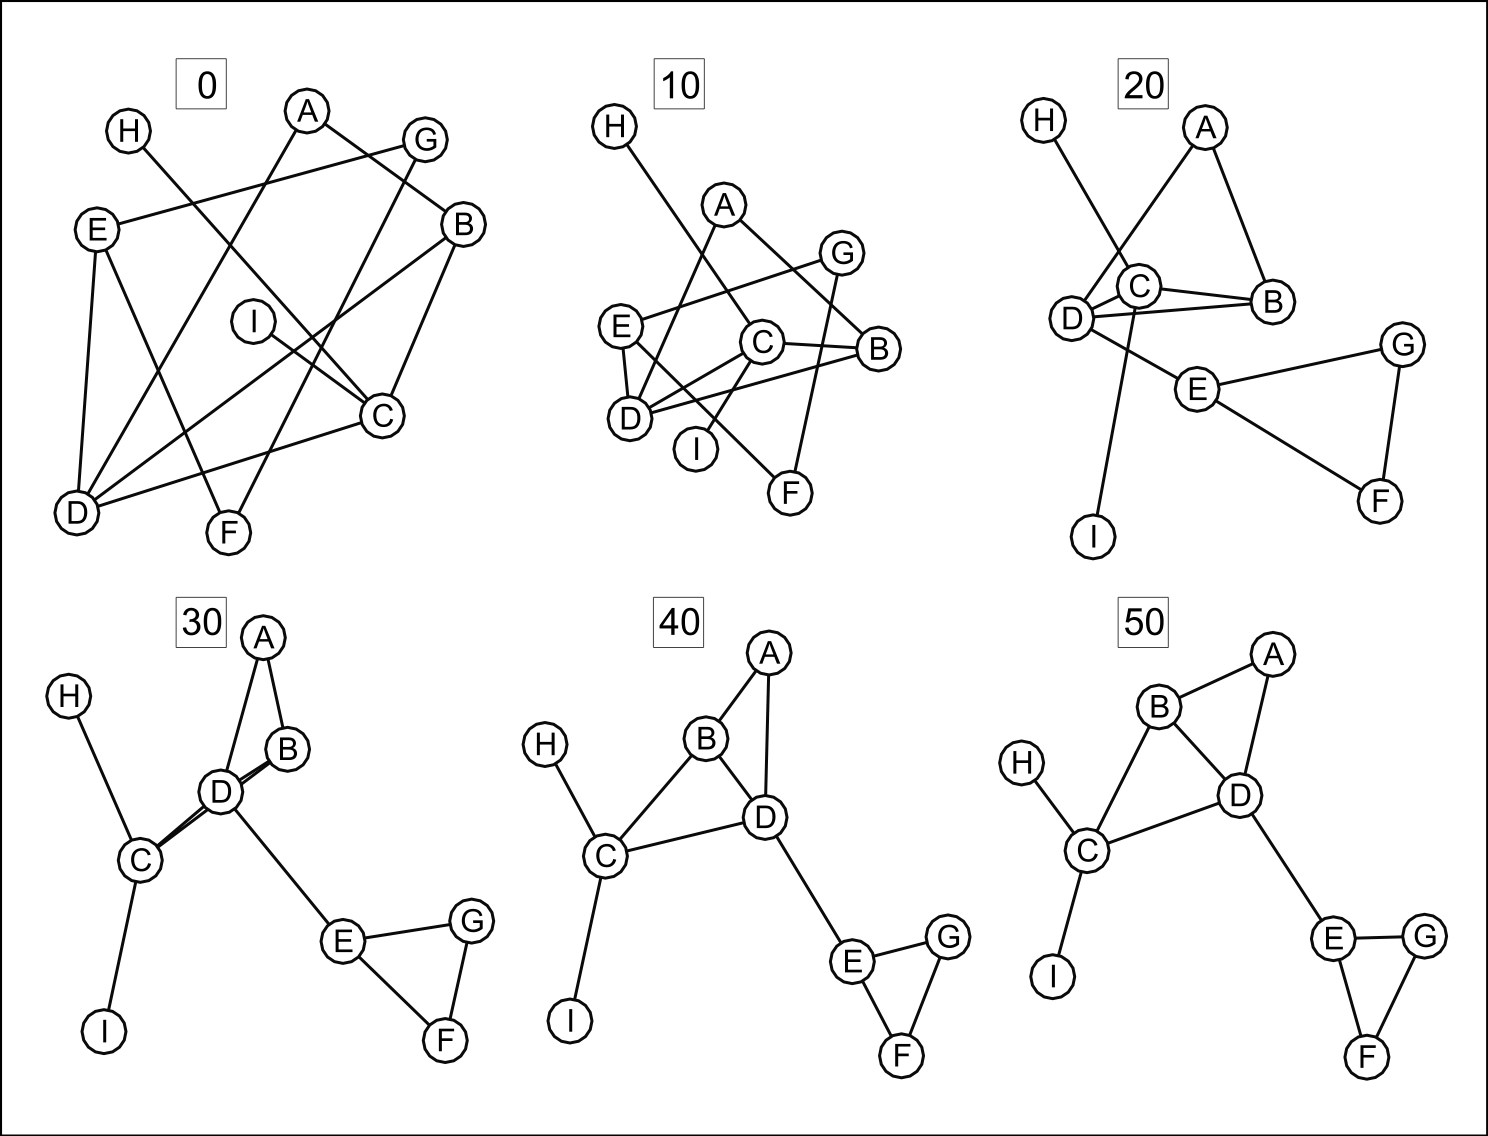
\includegraphics[width=\textwidth]{force-directed-layouts}
    \caption{Schrittweises Durchführen des Layout-Algorithmus von Fruchterman/Reingold}
    \bildquelle{Fruchterman, Thomas M. J./Reingold, Edward M.: Graph Drawing by Force-Directed Placement}
    \label{fig:force-directed-layouts}
\end{figure}

Force-Directed Layouts sind besonders effektiv für die übersichtliche
Darstellung von Netzwerken, in denen die Verbindungen zwischen den Elementen im
Vordergrund stehen. \parencite{force-directed-layouts} Im Gegensatz dazu
erfordert der Studiengangsfinder eine kontinuierliche Positionierung der
Studiengänge basierend auf inhaltlichen Ähnlichkeiten, was nicht unbedingt der
Stärke von Force-Directed Layouts entspricht. Force-Directed Graph Drawing
benötigt als Vorraussetzung bereits einen Graphen mit Knoten und Kanten, welche
im Fall des Studiengangsfinders die Ähnlichkeiten zwischen den einzelnen
Studiengängen entsprechen würde. Gerade die Berechnung der Ähnlichkeit zwischen
den einzelnen Studiengängen ist jedoch wesentlicher Bestandteil dieser Arbeit,
weshalb der Algorithmus nicht näher untersucht wurde.

\subsubsection{K-Means Clustering Algorithmus}
K-Means ist ein Clustering-Algorithmus, der Datenpunkte in k vordefinierte
Gruppen oder Cluster einteilt. Die Wahl von K stellt die Anzahl der Cluster dar,
und der Algorithmus versucht, die Datenpunkte so zu gruppieren, dass die Varianz
innerhalb der Cluster minimiert wird (siehe \autoref{fig:kmeans}).
\parencite{kmeans}

\begin{figure}[H]
    \centering
    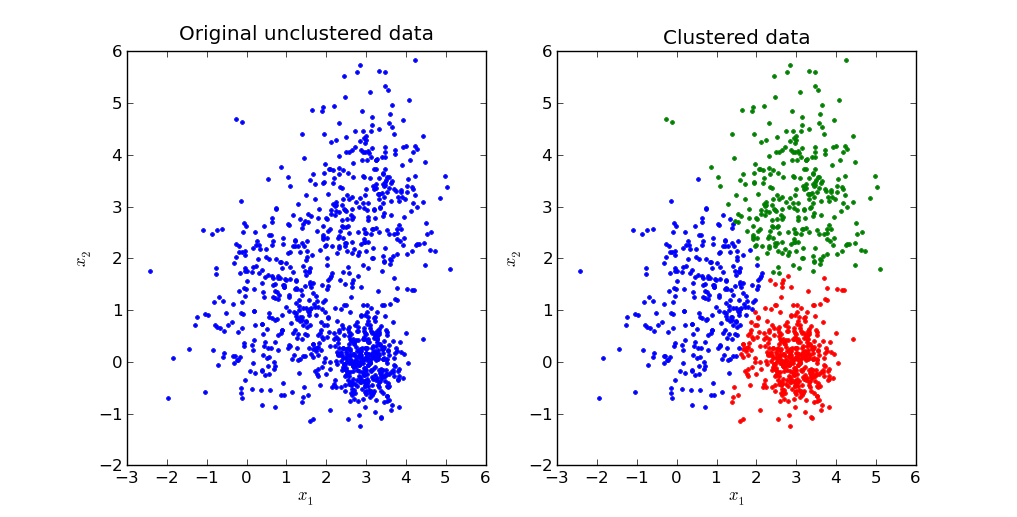
\includegraphics[width=\textwidth]{kmeans}
    \caption{K-Means Clustering Algorithmus}
    \bildquelle{https://mubaris.com/posts/kmeans-clustering/}
    \label{fig:kmeans}
\end{figure}

Die Entscheidung, den K-Means-Algorithmus nicht zu verwenden, basiert darauf,
dass dieser hauptsächlich darauf abzielt, Datenpunkte zu gruppieren und weniger
auf deren präzise Positionierung in einem zweidimensionalen Raum. Der
Algorithmus fordert außerdem eine vordefinierte Clusteranzahl k. Das stellt im
Falle des Studiengangsfinders jedoch keine Einschränkung dar, da jeder Cluster
eine Inhaltskategorie, wie zum Beispiel \glqq Informatik\grqq{} repräsentieren
würde. Trotzdem erweist sich der K-Means Clustering Algorithmus als unpassend,
da er sehr empfindlich gegenüber Ausreißern ist, da er versucht, Clusterzentren
zu finden, die die Gesamtvarianz minimieren. Wenn es Ausreißer in den
Studienschwerpunkten gibt, könnten sie das Ergebnis beeinflussen.
\parencite{kmeans-spikes}

Insgesamt erfüllt der MDS-Algorithmus die spezifischen Anforderungen des
Studiengangsfinders, indem er eine übersichtliche und interpretierbare
Visualisierung der Studiengänge basierend auf inhaltlichen Ähnlichkeiten
ermöglicht.

\subsubsection{Multidimensionale Skalierung (MDS)}\label{sec:MDS}
MDS ermöglicht die Reduktion $n$-dimensionaler Daten auf $m$-Dimensionen,
wodurch eine anschauliche Darstellung in Form von Koordinatenpaaren
ermöglicht wird \parencite{intro-to-multidimensional-scaling}. Dieser Aspekt ist
entscheidend, um Studiengänge in einem zweidimensionalen Diagramm zu
positionieren, wobei ähnliche Studiengänge aufgrund ihrer inhaltlichen
Ähnlichkeiten nahe beieinander liegen. Die Anwendung des MDS-Algorithmus auf
eine genormte Tabelle, in der im Falle von StudyMap die Studiengänge nach ihren
Anteilen an verschiedenen Inhaltskategorien gewichtet sind, ermöglicht eine
effektive Positionierung im Diagramm (siehe \autoref{table:input-mds}).

\begin{table}[!ht]
    \centering
    \begin{tabular}{|l|l|l|l|l|l|l|}
    \hline
        \textbf{Kürzel} & \textbf{Architektur} & \textbf{Gesundheit} & \textbf{Technik} & \textbf{Informatik} & \textbf{Wirtschaft} & \textbf{Internat.} \\ \hline
        \textbf{AT} & 0,55 & 0,06 & 0,09 & 0,04 & 0 & 0 \\ \hline
        \textbf{B} & 0,75 & 0 & 0 & 0,1 & 0 & 0,01 \\ \hline
        \textbf{ID} & 0,1 & 0,05 & 0,15 & 0,05 & 0,05 & 0 \\ \hline
        \textbf{HK} & 0,01 & 0,7 & 0,01 & 0,01 & 0,1 & 0,05 \\ \hline
        \textbf{PA} & 0 & 0 & 0,6 & 0,2 & 0,12 & 0,02 \\ \hline
        \textbf{IE} & 0 & 0 & 0,34 & 0,32 & 0,22 & 0,04 \\ \hline
        \textbf{LP} & 0 & 0,89 & 0,01 & 0 & 0,04 & 0,02 \\ \hline
        \textbf{SA} & 0 & 0,98 & 0 & 0 & 0 & 0 \\ \hline
        \textbf{IN} & 0 & 0 & 0,05 & 0,9 & 0 & 0,2 \\ \hline
        \textbf{IW} & 0 & 0 & 0,05 & 0,75 & 0,15 & 0,2 \\ \hline
        % \textbf{IM} & 0 & 0,2 & 0,1 & 0,65 & 0 & 0,05 \\ \hline
        % \textbf{BW} & 0 & 0 & 0 & 0 & 0,6 & 0,1 \\ \hline
        % \textbf{EB} & 0 & 0 & 0 & 0 & 0,5 & 0,4 \\ \hline
        % \textbf{SE} & 0 & 0 & 0,45 & 0,35 & 0,05 & 0,05 \\ \hline
        % \textbf{UI} & 0 & 0 & 0,36 & 0,12 & 0 & 0,04 \\ \hline
        % \textbf{MS} & 0 & 0 & 0,66 & 0,18 & 0 & 0,04 \\ \hline
        % \textbf{IR} & 0 & 0 & 0 & 0 & 0,1 & 0,8 \\ \hline
        % \textbf{REE} & 0 & 0 & 0,25 & 0,15 & 0,05 & 0,05 \\ \hline
        % \textbf{EI} & 0 & 0 & 0,5 & 0,25 & 0,05 & 0,05 \\ \hline
        % \textbf{ME} & 0 & 0 & 0,75 & 0,1 & 0,03 & 0,02 \\ \hline
        % \textbf{BE} & 0 & 0,07 & 0,6 & 0,12 & 0,11 & 0,06 \\ \hline
        % \textbf{MB} & 0 & 0 & 0,87 & 0,1 & 0,02 & 0 \\ \hline
        % \textbf{PT} & 0 & 0,95 & 0 & 0,03 & 0 & 0,09 \\ \hline
    \end{tabular}

    \caption{Exemplarische Eingabetabelle für den MDS-Algorithmus}
    \label{table:input-mds}
\end{table}

\autoref{table:input-mds} stellt eine stark vereinfachte Eingabetabelle für den
MDS-Algorithmus dar. Die erste Spalte enthält die Kürzel der verschiedenen
Studiengänge, wobei beispielsweise \textit{AT} für den Bachelor-Studiengang
Architektur steht. Die folgenden Spalten enthalten genormte Werte zwischen 0 und
1, die die prozentualen Anteile verschiedener Inhaltskategorien in den
jeweiligen Studiengängen repräsentieren. Diese genormten Werte werden im
n-dimensionalen Raum positioniert. Durch Anwendung des MDS-Algorithmus werden im
Verlauf die $n$-Dimensionen auf zwei Dimensionen reduziert, um schließlich eine
ästhetisch ansprechende Visualisierung in Form eines Diagramms zu generieren.

Der klassische MDS-Algorithmus besteht aus den folgenden vier Schritten
\parencite{mds-for-dimensionality-reduction}:

% https://ceopedia.org/index.php/Multidimensional_scaling
\paragraph*{1. Berechnung der Distanzmatrix $ D_{ij} $}\label{sec:distanzmatrix}
Die Berechnung der Distanzmatrix $ D_{ij} $ erfolgt mithilfe des euklidischen
Abstands zwischen den Studiengängen im n-dimensionalen Raum. Der euklidische
Abstand zwischen zwei Punkten $ P_{i} $ und $ P_{j} $ wird nach der Formel

$$ d(P_i, P_j) = \sqrt{(x_i - x_j)^2 + (y_i - y_j)^2 + \ldots + (z_i - z_j)^2} $$

berechnet, wobei $ x_{i} $, $ y_{i} $, ..., $ z_{i} $ die Koordinaten von Punkt
$ P_{i} $ im n-dimensionalen Raum sind \parencite{mds-ceopedia}. Für die
Studiengangsdaten bedeutet das, dass die n-Dimesionen die verschiedenen
Inhaltskategorien repräsentieren.

Die euklidische Distanzmatrix $ D_{ij} $ enthält dann die euklidischen Abstände
zwischen jedem Paar von Studiengängen. In der Matrix sind die Elemente
$ D_{ij} $ die Distanzen zwischen den Studiengängen $ i $ und $ j $. Je näher
die Studiengänge in der Distanzmatrix beieinander liegen, desto näher werden sie
im finalen Diagramm platziert und umgekehrt.

Konkret in Python implementiert, sieht die Berechnung der Distanzmatrix wie
folgt aus:

\begin{lstlisting}[style=Python]
def calculate_distance_matrix(X):
    euclidean = lambda x,y:ma.sqrt(np.sum((np.array(x)-np.array(y))**2))
    D = []
    for x in X:
        tmp = []
        for y in X:
            tmp.append(euclidean(x, y))
        D.append(tmp)
    return D
\end{lstlisting}

% https://dorianhe.github.io/Intro-to-Multidimensional-Scaling/
% https://ceopedia.org/index.php/Multidimensional_scaling
% https://www.hongfeili.com/files/paper100/paper4.pdf
\paragraph*{2. Anwendung der Centering Matrix $ C $ zur Normalisierung der
Distanzen}
Die Formel $ C = I - \frac{1}{n} \vec{e} * \vec{e}^T $ berechnet die
sogenannte Centering Matrix. $ I $ ist die Einheitsmatrix, $ \frac{1}{n} $ ist
der Kehrwert der Anzahl der Datenpunkte und $ \vec{e} $ ist ein Vektor gefüllt
mit Einsen. Das Symbol $ \vec{e}^T $ bezeichnet wie üblich die Transposition
des Vektors. \parencite{an-introduction-to-mds}

Die Centering Matrix $ C $ wird verwendet, um die Distanzmatrix $ D $ zu
zentrieren. Das Zentrieren ist wichtig, um die Distanzen zwischen den Punkten
in der n-dimensionalen Raummatrix zu normieren und somit den Schwerpunkt der
Daten im Raum zu korrigieren. \parencite{an-introduction-to-mds}

Schließlich wird diese eingesetzt um die Zentriermatrix $ B $ aus der
Distanzmatrix zu berechnen:
$$ B = - \frac{1}{2} * C * D_{ij} * C $$

\paragraph*{3. Spektralzerlegung}
Die Matrix $ B $ wird nun spektral zerlegt, um die Eigenwerte $ \lambda_{i} $
und die zugehörigen Eigenvektoren $ v_{i} $ zu erhalten.
$$ B = W * \Lambda * W^-1 $$
Hierbei ist $ W $ die Matrix der Eigenvektoren und $ \Lambda $ ist eine
Diagonalmatrix mit den Eigenwerten auf der Hauptdiagonale. Die Eigenvektoren
werden anschließend sortiert und die größten positiven Eigenwerte
$ \lambda_{1} ... \lambda{m} $ mit dazugehörigen Eigenvektoren
$ v_{1} ... v_{m} $ aus B extrahiert. \parencite{an-introduction-to-mds}

\paragraph*{4. Projektion der Datenpunkte}
Um nun die Datenpunkte von einem höherdimensionalen Raum (basierend auf den
Beziehungen in der Distanzmatrix $ D $) auf einen niedrigdimensionalen Raum,
der durch die Eigenvektoren und Eigenwerte repräsentiert wird, abzubilden,
benötigt man folgende Projektion \parencite{intro-to-multidimensional-scaling}:
$$ X = V_m \Lambda^{1/2}_m $$
Die Variable $ m $ steht für die Anzahl der gewünschten Dimensionen. Im Falle
von StudyMap entspricht $ m = 2 $, um das Ergebnis in einem 2D-Diagramm zu
visualisieren. $ V_{m} $ steht für die Eigenvektoren und $ \Lambda $ wie bereits
im vorherigen Absatz beschrieben für die Diagonalmatrix mit den Eigenwerten.
\parencite{an-introduction-to-mds}

Abschließend enthält $ X $ die Matrix mit den auf $ m $-Dimensionen reduzierten
Koordinaten, welche dann z.B. in einem Diagramm visualisiert werden können.
An dieser Stelle wird für die Berechnung der Studiengänge (mit $ m = 2 $)
ermöglicht, dass innerhalb einer 2D-Darstellung, ähnliche Studiengänge aufgrund
ihrer inhaltlichen Ähnlichkeiten nahe beinander positioniert werden. Diese
räumliche Anordnung erleichtert die intuitive Analyse von Beziehungen zwischen
den einzelnen Bachelor- und Masterstudiengängen.

\subsection{Auswahl der Technologien}
Die Auswahl der geeigneten Technologien für die Entwicklung des innovativen 
Studiengangsfinders wurde sorgfältig überlegt, um eine effiziente und
interaktive Lösung zu gewährleisten. Besonders wichtig ist die Nutzbarkeit auf
Smartphones und Desktop-Geräten, wodurch sich außerdem neue Herausforderungen
hinsichtlich der Bedienung ergeben. Im Folgenden werden die Hauptkomponenten des
Technologiestacks und ihre jeweiligen Funktionen erläutert.

\subsubsection{Interaktive Grafik (Frontend)}
Für die Darstellung der interaktiven Grafik wurde Pixi.js gewählt. Pixi.js ist
ein leistungsstarkes WebGL-Rendering-Framework, das eine schnelle und
reibungslose Darstellung von Grafiken ermöglicht. \parencite{pixijs} Die
Entscheidung für Pixi.js basiert auf seiner Effizienz bei der Verarbeitung
komplexer 2D-Grafiken und seiner Fähigkeit, eine ansprechende Benutzererfahrung
zu bieten.

Neben Pixi.js wurden verschiedene weitere Bibliotheken betrachtet:
\begin{itemize}
    \item three.js: WebGL 3D-Framework
    \item D3.js: 2D-Datenvisualisierungsbibliothek
    \item Chart.js: HTML5-Bibliothek für Diagramme
    \item Paper.js: HTML5-Bibliothek für Animationen und interaktive Grafiken
    \item Fabric.js: 2D-Canvas Bibliothek
\end{itemize}

% TODO: Quellen für die "Forenthreads" gegen die Frameworks etc verlinken

Der Studiengangsfinder erfordert eine 2D-Grafikdarstellung, weshalb
\textit{three.js}, das auf 3D-Visualisierungen spezialisiert ist, nicht als
geeignete Grundlage gewählt wurde. \parencite{threejs}

Die Entscheidung gegen die Verwendung von \textit{D3.js} wurde aufgrund
von Bedenken bezüglich der Dokumentation und der Wahrnehmung in der 
Entwicklergemeinschaft getroffen. Die unvollständige Dokumentation und
bestehende Forenthreads, die die Relevanz von D3.js in Frage stellen, könnten zu
potenziellen Schwierigkeiten bei der Entwicklung und zukünftigen Wartungen
führen. \parencite{d3js}

% d3js-trend, d3js-trend-2

Aufgrund der festgestellten Einschränkungen in der Flexibilität von
\textit{Chart.js} wurde gegen die Verwendung der Bibliothek entschieden. Obwohl
Chart.js die Erstellung einer Vielzahl von Diagrammen ermöglicht, hat sich
gezeigt, dass die Anpassbarkeit eingeschränkt ist. \parencite{chartjs}

Basierend auf der wahrgenommenen Inaktivität des Projekts und den festgestellten 
Einschränkungen in Bezug auf Event-Handler wurde entschieden, \textit{Paper.js}
nicht zu verwenden. \parencite{paperjs} Die begrenzten Event-Handler schränken
die Interaktionsmöglichkeiten ein, was im Kontext des Studiengangsfinders, der
eine umfassende Benutzerinteraktion für Smartphone und Desktop-Gerät erfordert,
als unzureichend erachtet wurde. \parencite{paperjs-events}

Obwohl \textit{Fabric.js} als vielversprechende Alternative erschien, wurde
Pixi.js aufgrund mehrerer Faktoren bevorzugt \parencite{fabricjs}. Der
professionellere Website-Auftritt von Pixi.js trug dazu bei, das Vertrauen in
die Zuverlässigkeit und Wartbarkeit des Frameworks zu stärken. Ein weiterer
bedeutender Punkt ist die Anzahl der GitHub-Sterne in Relation zu der Anzahl an
\textit{offenen Issues}, die Pixi.js aufweist. Eine höhere Anzahl an
GitHub-Sternen mit gleichzeitig weniger offenen Issues, deutet oft auf eine
größere und aktivere Entwicklergemeinschaft hin, was wiederum auf
kontinuierliche Weiterentwicklung und Wartung schließen lässt.
\parencite{paperjs-pixijs-comparison}

\subsubsection{Berechnung der Positionen (Backend)}
Die Berechnung der Positionen für die Studiengänge basiert, wie im Abschnitt
\ref{sec:MDS} erläutert, auf dem Multidimensionalen Skalierungsalgorithmus
(MDS), der in Python implementiert ist. Der Algorithmus verarbeitet eine
strukturierte CSV-Datei, die alle relevanten Informationen zu den Studiengängen,
Feldern und Meta-Informationen (wie z.B. Fakultätszugehörigkeit) enthält. Dieser
Datensatz bildet die Grundlage für die Positionsbestimmung im zweidimensionalen
Raum.

Hierzu wird ein Python-Skript entwickelt, welches die CSV-Datei einliest und
schließlich den MDS-Algorithmus auf den Daten anwendet. Im Verlauf der
Arbeit wurde eine anfängliche Eigenimplementierung des MDS-Algorithmus in
Betracht gezogen. Folgender Ausschnitt eines Quellcodes beinhaltet die für diese
Arbeit entwickelte Eigenimplementierung, basierend auf dem im Abschnitt
\ref{sec:MDS} genau erläuterten Ablauf:

\begin{lstlisting}[style=Python]
    import numpy as np

    def calculate_distance_matrix(X):
        ...

    def read_data_from_csv():
        ...

    def mds(self):
        # Reads data from CSV file and transforms it to number rows
        X = self.read_data_from_csv()

        # Calculates distance matrix
        M = self.calculate_distance_matrix(X)

        # Double centered matrix
        n = 11 # Number of subjects
        I = np.identity(n) # Identity matrix
        Jn = np.ones((n, n)) # Matrix Jn of all ones
        C = I - (1/n) * Jn # Calculate centering matrix C
        B = -0.5 * np.dot(np.dot(C, np.array(M)), C) # Calculate the double centered matrix B

        # Eigenvalues, Eigenvectors
        m = 2  # number of dimensions (2D)
        eigenvalues, eigenvectors = np.linalg.eig(B) # Perform eigenvalue decomposition

        # Sort eigenvalues and corresponding eigenvectors in descending order
        sorted_indices = np.argsort(eigenvalues)[::-1]
        eigenvalues = eigenvalues[sorted_indices]
        eigenvectors = eigenvectors[:, sorted_indices]

        # Select the top m eigenvalues and corresponding eigenvectors
        top_m_eigenvalues = eigenvalues[:m]
        top_m_eigenvectors = eigenvectors[:, :m]

        # Calculate the square root of the diagonal matrix
        sqrt_Lambda_m = np.sqrt(np.diag(top_m_eigenvalues))

        # Compute the matrix X using the formula
        X_transformed = np.dot(top_m_eigenvectors, sqrt_Lambda_m)

        return X_transformed
\end{lstlisting}

Die Methode \code{calculate\_distance\_matrix} berechnet die Distanzmatrix,
welche für den Ablauf des Programms essenziell ist. Der Code dazu wird an
dieser Stelle ausgespart, da er bereits in Abschnitt \ref{sec:distanzmatrix}
vollständig spezifiziert wurde. Außerdem ausgespart ist die Methode
\code{read\_data\_from\_csv()}, welche die Eingabedatei einliest, analysiert und
schließlich die zur Berechnung benötigten Zahlen-Arrays zurückgibt. Wie in Zeile
1 des Quellcodes ersichtlich, wird zur Berechnung der mathematischen Gleichungen
die Programmbibliothek NumPy verwendet. \parencite{numpy}

Die Entwicklung und Umsetzung dieser eigenen Lösung erwies
sich jedoch als äußerst anspruchsvoll, da sie zahlreiche subtile mathematische
Nuancen berücksichtigen müsste. Angesichts dieser Komplexität wurde die
Entscheidung getroffen, auf die bewährte und leistungsstarke
SciKit-Learn-Bibliothek zurückzugreifen. Die Verwendung dieser etablierten
Implementierung ermöglicht eine präzise und effiziente Lösung, wobei der Fokus
auf den zentralen Fragestellungen der Masterarbeit liegt. Außerdem gewährleistet
die Einbindung von SciKit-Learn neben der Robustheit der MDS-Umsetzung, auch die
Reduktion der Entwicklungskomplexität im Hinblick auf die
Algorithmusimplementierung. \parencite{scikit-learn}

Das Ergebnis des Skripts sind Koordinaten für jeden Studiengang im
zweidimensionalen Raum. Diese Koordinaten werden anschließend zusammen mit den
vorher eingelesenen Meta-Daten zu den Studiengängen in JSON-Dateien gespeichert,
die schließlich vom Backend über eine REST-API bereitgestellt werden.

Neben dem Python-Programm besteht das Backend außerdem aus einem Node.js-Server,
der mithilfe von der Bibliothek Express erstellt wurde. Node.js ist eine
JavaScript-Runtime-Umgebung, die auf der V8 JavaScript Engine von Google basiert
und eine serverseitige Ausführung von JavaScript ermöglicht. \parencite{nodejs}
Express wiederum ist ein quelloffenes Webanwendungs-Framework für Node.js. Es
erleichtert die Erstellung von Webanwendungen und APIs, indem es eine Reihe von
Funktionen und Tools für den Aufbau von Webanwendungen bereitstellt.
\parencite{express}

Der daraus entstehende Webservice ermöglicht den Zugriff, auf die vom
Python-Skript generierten Dateien, über standardisierte RESTful Endpunkte. Durch
diese API kann das Frontend in Echtzeit die benötigten Informationen abrufen, um
die interaktive Grafik der Studiengänge zu erstellen. Die klare Trennung von
Backend und Frontend gewährleistet eine effiziente Datenübertragung und
ermöglicht eine dynamische Aktualisierung der Grafik bei Änderungen im
Datensatz.

Der Vorteil bei der Speicherung der Daten in Form von JSON-Dateien liegt darin,
dass die Daten wesentlich seltener geändert werden, als die Website aufgerufen
wird. Somit wird effektiv Rechenleistung und Strom gespart. Gleichzeitig erhöht
dieses Vorgehen die Performance der Website. Zur Festigung dieser These werden
die Google Suchtrends von 2021 zum Suchbegriff \glqq OTH Regensburg
Studiengänge\grqq{} herangezogen (siehe Anhang
\ref{appendix:google-search-trends}). Die Trends zeigen eine Jahressumme von
1194 Suchanfragen. Die Anzahl an Suchanfragen lassen sich offensichtlich nicht
1:1 in Seitenaufrufe projezieren, verdeutlichen aber dennoch einen ungefähren
Richtwert. Die Datengenerierung hingegen wird nur bei größeren Änderungen an den
Inhalten von Studiengängen, oder beim Hinzufügen bzw. Entfernen eines 
Studiengangs ausgelöst.